%% Præsentation for C-programmering for begyndere
%% Lavet af Jacob Bechmann Pedersen og Jacob Skjødt Nielsen
%% For C undervisning i IDA 
%%
%% Theme: `DarkConsole'
%% Copyright (c) 2011-2017 Kazuki Maeda <kmaeda@kmaeda.net>
%% Distributable under the MIT License:
%% http://www.opensource.org/licenses/mit-license.php 

%% Preamble
\documentclass{beamer}

\usepackage{hyperref} % Add a link to your document
\usepackage{graphicx} % Add pictures to your document
\usepackage{listings} % Source code formatting and highlighting
\usepackage[utf8]{inputenc} % Gives UTF-8 encoded characters such as Æ, Ø, Å.

%% Setting the C language type, for viewing pleasure:
\usepackage{listings}
\usepackage{color}

\definecolor{link}{HTML}{CF55E3}
\definecolor{dkgreen}{rgb}{0,0.6,0}
\definecolor{gray}{rgb}{0.5,0.5,0.5}

\lstset{frame=tb,
  inputencoding=utf8,
  language=C,
  aboveskip=3mm,
  belowskip=3mm,
  showstringspaces=false,
  columns=flexible,
  basicstyle={\small\ttfamily},
  numbers=left,
  numbersep=0pt,
  keywordsprefix={\#, \<},
  numberstyle=\tiny\color{gray},
  keywordstyle=\color{C_darkblue},
  commentstyle=\color{dkgreen},
  stringstyle=\color{C_lightblue},
  breaklines=true,
  breakatwhitespace=true,
  tabsize=3,
  extendedchars=true,
  literate={æ}{{\ae}}1 {ø}{{\o}}1 {å}{{\r a}}1 {Æ}{{\AE}}1 {Ø}{{\O}}1 {Å}{{\r A}}1,
}

\usetheme{C_Console}
\title{C-Programmering for begyndere}
\date{16. april 2018}
\subtitle{Del 3 - Funktioner, arrays, datarepræsentationer}
\author{Jacob B. Pedersen\footnote{jacob.bp@mvb.net} og Jakob S. Nielsen\footnote{jakob990@gmail.com}}

%% Document
\begin{document}

\begin{frame}
	\maketitle
\end{frame}

\begin{frame}{Indhold}
	\tableofcontents
\end{frame}

\section{Repetition}
%%----------------------------------------------------------------------
\subsection{Hvad lavede vi sidste gang?}

\begin{frame}[fragile]{Hvad lavede vi sidste gang?}
	\begin{itemize}
		\item{Vi gennemgik operatorer, og deres betydning for if-else statements:}
		\begin{lstlisting}
		if([betingelse]){
			handling();
		}
		else if({betingelse2]){
			handling2();
		}
		else{
			handling3();
		}
		\end{lstlisting}
	\end{itemize}
\end{frame}

%----------------------------------------------------------------------

\begin{frame}[fragile]{Hvad lavede vi sidste gang?}
	\begin{itemize}
		\item{Operatorerne selv evalueredes blot til Boolske udtryk som {\color{dkgreen}true} og {\color{dkgreen}false}:}
		\begin{lstlisting}
		1 > 2; // false
		3 >= 3; // true
		12 > 2 && 12 < 11; // false
		12 > 2 || 12 < 11; // true
		\end{lstlisting}
	\end{itemize}
\end{frame}


%----------------------------------------------------------------------

\begin{frame}[fragile]{Hvad lavede vi sidste gang?}
	\begin{itemize}
		\item{På samme måde kunne de også bruges som betingelser i løkkerne}
		\item{Her var der {\color{C_darkblue}while}() og {\color{C_darkblue}for}() -løkkerne:}
		\begin{lstlisting}
		int i = 0;
		while(i <= 10){
			printf(”%d”, i);
			i++;
		}

		for(int j = 0; j <= 10, j++){
			printf(”%d”, j);
		}
		\end{lstlisting}
	\end{itemize}
\end{frame}

%----------------------------------------------------------------------

\begin{frame}[fragile]{Hvad lavede vi sidste gang?}
	\begin{itemize}
		\item{Til sidst kiggede vi på {\color{C_darkblue}switch}-cases:}
		\begin{lstlisting}
		switch(variabel)
		{
			case 1:
			handling();
			break;

			case 2:
			andenHandling();
			break;

			default:
			break;
		}
		\end{lstlisting}
	\end{itemize}
\end{frame}

\section{I dag}
%%----------------------------------------------------------------------
\subsection{Dagens program}

\begin{frame}[fragile]{Dagens program}
	\begin{itemize}
		\item{I dag kigger vi på mere avanceret brug af C:}
		\item{Funktioner}
		\begin{itemize}
			\item{Genopfriske argumenter og retur-værdier}
			\item{Header- og implementationsfiler}
			\item{Hvad skal der til for at lave et library?}
		\end{itemize}
		\item{Arrays}
		\begin{itemize}
			\item{Lister over variable, refereret til ved indeks}
			\item{Nogle af jer har forsøgt sig med char array AKA strings}
		\end{itemize}
		\item{Anderledes datarepræsentation:}
		\begin{itemize}
			\item{{\color{C_darkblue}typedef} og {\color{C_darkblue}enum}}
			\item{Klynger af data i {\color{C_darkblue}structs}}
			\item{Flerformet data i {\color{C_darkblue}unions}}
		\end{itemize}
	\end{itemize}
\end{frame}

%%----------------------------------------------------------------------
\subsection{Funktioner}

\begin{frame}[fragile]{Funktioner}
	\begin{itemize}
		\item{Vi har ofte brugt funktioner:}
		\begin{itemize}
			\item{{\color{C_darkblue}pow}(), {\color{C_darkblue}sqrt}(), {\color{C_darkblue}rand}(), {\color{C_darkblue}printf}() og {\color{C_darkblue}scanf}()}
		\end{itemize}
		\item{De ligner alle i skrift lidt matematiske funktioner:}
		\begin{equation}
      	printf(x)
    		\end{equation}
    		\item{Og vi kan selvfølgelig også designe vores egne!}
    		\item{Vi husker tydeligt en funktionsdefinition, vi har med hver gang:}
    		\begin{lstlisting}
		int main(int argc, char ** argv){
			return 0;
		}
		\end{lstlisting}
	\end{itemize}
\end{frame}

%%----------------------------------------------------------------------

\begin{frame}[fragile]{Funktioner}
	\begin{itemize}
		\item{I funktionerne er der en række begrber vi skal genopfriske/kende:}
		\begin{itemize}
			\item{{\color{dkgreen}returtype}, {\color{dkgreen}argumenttype/parameter}, {\color{dkgreen}returværdi} og {\color{dkgreen}lokale variable}:}
		\end{itemize}
	\begin{center}
		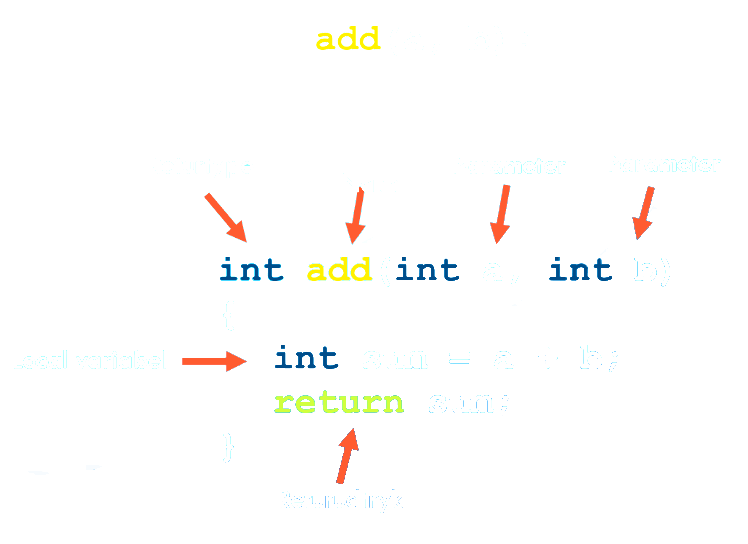
\includegraphics[width=0.7\textwidth]{assets/function_description.png}
	\end{center}
	\end{itemize}
\end{frame}

%%----------------------------------------------------------------------

\begin{frame}[fragile]{Funktioner}
	\begin{itemize}
		\item{Så først defineres funktionen, og derefter  kan den kaldes som alt andet i main:}
		\begin{lstlisting}
		int add( int a, int b ){
			int result = a + b;
			return result;
		}

		int main(void){
			int a = 3;
			int b = 2;
			printf(”%d + %d = %d”, a, b, add(a,b));
		}
		\end{lstlisting}
	\end{itemize}
\end{frame}

%%----------------------------------------------------------------------

\begin{frame}[fragile]{Funktioner}
	\begin{itemize}
		\item{Noget andet fedt man kan med sine funktioner, er at kalde dem rekursivt:}
		\begin{lstlisting}
		int rekursion(int antalGange){
			if(antalGange < 0){
			return 0;
			}
			printf(”%d”, rekursion(antalGange-1));
			return antalGange;
		}
		\end{lstlisting}
		\item{Man skal bare huske at sikre at computeren kan komme ud af de rekursive kald igen}
		\item{Ellers risikerer man et:}
		\begin{center}
		
\includegraphics[width=0.7\textwidth]{assets/so-logo.png}
	\end{center}
	\end{itemize}
\end{frame}

%%----------------------------------------------------------------------

\begin{frame}[fragile]{Funktioner}
	\begin{itemize}
		\item{Vi har berørt libraries lidt før:}
		\begin{itemize}
			\item{{\color{dkgreen}stdio.h}, {\color{dkgreen}math.h}, {\color{dkgreen}stdbool.h}}
			\item{De er alle sammen standard libraries}
			\item{Er enten en del af compileren eller operativsystemet}
		\end{itemize}
		\item{Men vi kan sagtens lave vores egne!}
		\begin{itemize}
			\item{Kræver blot en header-fil og implementationsfil:}
			\item{{\color{C_lightblue}library.h} og {\color{C_lightblue}library.c}}
			\item{Headeren er hvor vi deklarerer (/prototyper) vores variable og funktioner}
			\item{Implementationsfilen er til at beskrive den specifikke funktionalitet}
		\end{itemize}
	\end{itemize}
\end{frame}

%%----------------------------------------------------------------------

\begin{frame}[fragile]{Funktioner}
	\begin{itemize}
		\item{Eksempel på en header:}
		\begin{lstlisting}
		// Header skrives med "include guard" og instantierer funktionerne:
		#ifndef LIBRARY_H
		#define LIBRARY_H

		int add(int x, int y);

		#endif /* LIBRARY_H */
		\end{lstlisting}
		\item{Eksempel på en implementation:}
		\begin{lstlisting}
		// Inplementationen inkluderer headeren, og beskriver funktionerne:
		#include "library.h"
		
		int add (int x, int y){
			int sum = x + y;
			return sum;
		}
		\end{lstlisting}
	\end{itemize}
\end{frame}

%%----------------------------------------------------------------------
\subsection{Arrays}

\begin{frame}[fragile]{Arrays}
	\begin{itemize}
		\item{Vi har allerede stiftet bekendtskab med char arrays i opgavesæt 1}
		\item{Den opfører sig som en liste af chars, og man kan bruge den således:}
		\begin{lstlisting}
		char inputstring[LENGTH]; // Angiv længden af arrayet, så computeren kan sætte pladsen til side!
		scanf(”%s”, &inputString); // scanner efter en string indtil første mellemrum, newline etc.
		\end{lstlisting}
		\item{Det var der en del der fik til at fungere!}
		\item{Hvordan ser computeren så de data?}
		\begin{center}
		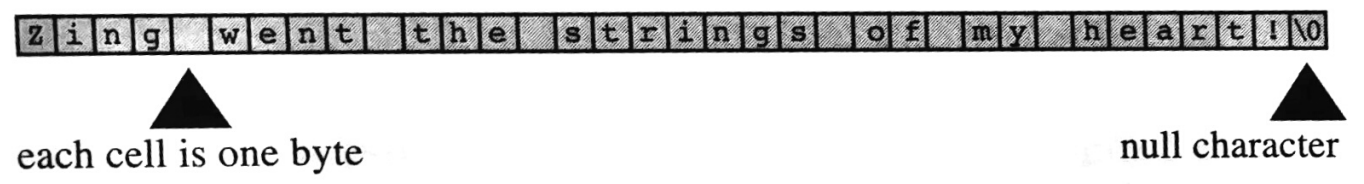
\includegraphics[width=0.7\textwidth]{assets/char_array.png}
		\end{center}
	\end{itemize}
\end{frame}

%%----------------------------------------------------------------------

\begin{frame}[fragile]{Arrays}
	\begin{itemize}
		\item{Vi har allerede stiftet bekendtskab med char arrays i opgavesæt 1}
		\item{Den opfører sig som en liste af chars, og man kan bruge den således:}
		\begin{lstlisting}
		char inputstring[LENGTH]; // Angiv længden af arrayet, så computeren kan sætte pladsen til side!
		scanf(”%s”, &inputString); // scanner efter en string indtil første mellemrum, newline etc.
		\end{lstlisting}
		\item{Det var der en del der fik til at fungere!}
		\item{Hvordan ser computeren så de data?}
		\begin{center}
		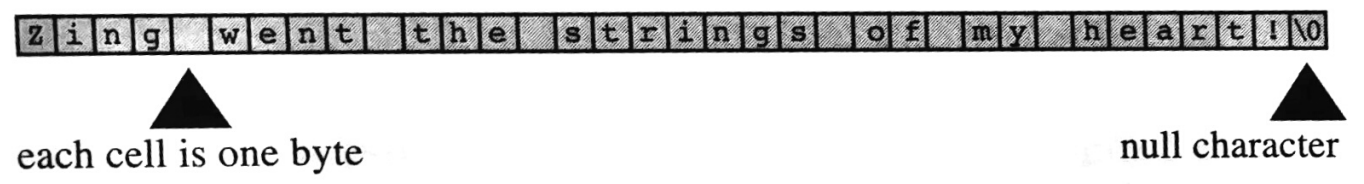
\includegraphics[width=0.7\textwidth]{assets/char_array.png}
		\end{center}
	\end{itemize}
\end{frame}

%%----------------------------------------------------------------------

\begin{frame}[fragile]{Arrays}
	\begin{itemize}
		\item{Char arrays er klart en oplagt brugt af denne type "lister"}
		\item{Men der findes arrays af alle typer:}
		\begin{lstlisting}
		// F.eks. en integer array:
		int heltal[] = {0, 1, 2, 3, 4, 5, 6, 7, 8, 9, 10};
		// Eller float array:
		float kommatal[] = {0.1, 1.5, 2.46, 3.23, 4.44, 5.71, 6.66, 7.91, 8.0, 9.11, 10.4};
		\end{lstlisting}
		\item{Der findes andre måder at opstille sådanne lister f.eks. dynamisk};
		\item{det er dog et avanceret emne, med skjulte fælder!}
		
	\end{itemize}
\end{frame}
		
%%----------------------------------------------------------------------

\begin{frame}[fragile]{Arrays}
	\begin{itemize}
		\item{Når man tilgår array elementer, sker det vha. indeks:}
		\begin{lstlisting}
		// Her på en string:
		char string[] = ”Zing went the string of my heart!”;
		printf(”%c”, string[0]);
		// Vil printe værdien 'Z'. 
		\end{lstlisting}
		\item{Altså er arrays 0-indekserede!}
		\item{men deres størrelse er angivet i antal elementer!, minimum 1! som får indeks 0}
	\end{itemize}
\end{frame}

%%----------------------------------------------------------------------
\subsection{typedef}

\begin{frame}[fragile]{typedefs og enums}
	\begin{itemize}
		\item{Hvad så med data der ikke er overskueligt i formen int, float osv.?}
		\item{Her kan {\color{C_darkblue}typedef} redde os:}
		\begin{lstlisting}
		// Et smart eksempel kunne være at gøre en fysisk udregning overskuelig:
		typedef float length;
		typedef float width;
		typedef float height;
		typedef float volume;
		// Det er altid vigtigt at koden er læselig for beskueren!
		length l = 23;
		width w = 32.5;
		height h = 55;
		volume v = l * w * h;
		\end{lstlisting}
	\end{itemize}
\end{frame}

%%----------------------------------------------------------------------
\subsection{enum}

\begin{frame}[fragile]{typedefs og enums}
	\begin{itemize}
		\item{Modsvar til {\color{C_darkblue}typedef}, {\color{C_darkblue}enum} bruges til at navngive værdier i stedet for datatyper
		\begin{lstlisting}
		// Hvis man skriver dem således, bliver de fortløbende nummereret fra 0:
		enum color { red, orange, yellow, green, blue, purple };
		// Ellers kan man selv bestemme hvad talværdi de har tilknyttet:
		enum color { red = 3, orange = 4, yellow = 0, green = 1, blue = 2, purple = 2 };
		
		// Variable af enum typen deklareres/initialiseres således:
		enum color favouriteColor = purple;
		\end{lstlisting}
		\item{Man kan også bruge {\color{C_darkblue}enum} med switch-cases!}
	\end{itemize}
\end{frame}

\section{Kreative Opgaver}
%%----------------------------------------------------------------------
\begin{frame}{Kreative Opgaver}
	\begin{itemize}
	\item{Det var det for nu!}
	\item{Der ligger som sidst kreative opgaver tilgængelige:}
		\begin{itemize}
		\item{\color{link}\href{https://github.com/Iakop/C-Programmering-for-begyndere/tree/master/Del_2/Exercises/C_exercises_2_dansk.pdf}{../Del\_2/Exercises/C\_exercises\_2\_dansk.pdf}}
		\end{itemize}
	\item{Der er hjælp at hente her på workshoppen}
	\item{God arbejdslyst! - Happy Hacking!}
	\end{itemize}
\end{frame}



\end{document}

%%\begin{frame}[fragile]
	%%\begin{lstlisting}
		%%#include <stdio.h>

		%%int main(void)
		%%{
		%%printf("Hello world\n");
		%%return 0;
		%%}
	%%\end{lstlisting}
%%\end{frame}